\documentclass[conference]{IEEEtran}

\IEEEoverridecommandlockouts

\usepackage{amsmath,amssymb,amsfonts, bbold}
\usepackage{hyperref}
\usepackage{algorithm, algpseudocode}
\usepackage{graphicx, multirow, hhline, pgfplots}
\pgfplotsset{compat=1.18}
\usepackage{comment}

\usepackage[citestyle=numeric,bibstyle=numeric,sorting=none,maxnames=10]{biblatex}
\addbibresource{biblio.bib}
\AtBeginBibliography{\small}

\makeatletter

\newcommand{\newlineauthors}{%
\end{@IEEEauthorhalign}\hfill\mbox{}\par
\mbox{}\begin{@IEEEauthorhalign}}  

\def\hlinewd#1{%
\noalign{\ifnum0=`}\fi\hrule \@height #1 %
\futurelet\reserved@a\@xhline}

\makeatother

\begin{document}

\title{Learning Observation Model for SLAM via Random Fourier Features in a Kernel Kalman Filter}

\author{
    \IEEEauthorblockN{HUBERT Bastien}
    \IEEEauthorblockA{\textit{DTIS, ONERA, Université Paris-Saclay} \\
    Palaiseau, France \\
    bastien.hubert@onera.fr}
\and
    \IEEEauthorblockN{DAHIA Karim}
    \IEEEauthorblockA{\textit{DTIS, ONERA, Université Paris-Saclay} \\
    Palaiseau, France \\
    karim.dahia@onera.fr}
\newlineauthors
\and
    \IEEEauthorblockN{MERLINGE Nicolas}
    \IEEEauthorblockA{\textit{DTIS, ONERA, Université Paris-Saclay} \\
    Palaiseau, France \\
    nicolas.merlinge@onera.fr}
\and
    \IEEEauthorblockN{GIREMUS Audrey}
    \IEEEauthorblockA{\textit{IMS, Université de Bordeaux, CNRS, Bordeaux INP} \\
    Talence, France \\
    audrey.giremus@u-bordeaux.fr}
}

\maketitle

\begin{abstract}
This paper addresses the problem of simultaneous localisation and mapping with an unknown observation model by formulating the navigation equations in reproducing kernel Hilbert spaces. This representation allows non-linearities to be handled through a Kalman-like recursion without explicit linearisations. Conjointly, the Hilbert space formulation is exploited to iteratively learn the observation model using a finite-dimensional random feature approximation, whose parameters are updated via recursive least squares minimisation. 

The resulting algorithm preserves the prediction–update structure of Bayesian filtering while learning the environment model alongside the state estimation. Simulation results on a non-linear navigation scenario and comparison to a generic particle filter provided with a degraded observation function show that the proposed approach consistently estimates its state while reconstructing an accurate observation model.
\end{abstract}

\section{Introduction}

Simultaneous Localisation and Mapping (SLAM) is a fundamental problem in autonomous navigation, in which an agent must concurrently build a map of an unknown environment and estimate its own position relative to that map. This problem has been extensively studied over the past two decades \cite{bib:tuto_SLAM,bib:Proba_robots}. Traditional navigation approaches are typically described by probabilistic state-space models in which both the motion and observation processes are explicitly defined. Under Gaussian assumptions and moderate non-linearities, Kalman filtering techniques provide computationally efficient solutions \cite{bib:UKF}. In contrast, particle filter-based methods relax linearisation assumptions and improve robustness at the cost of potential sample degeneracy in high-dimensional spaces \cite{bib:tuto_PF}.

A key assumption underlying these formulations is the availability of an accurate observation model. In practice, however, such a function may involve complex, poorly parameterised, or unknown physical mechanisms. Visual SLAM \cite{bib:visual_SLAM} or landmark-based SLAM \cite{bib:FastSLAM} algorithms rely on geometric features observable at a distance, reducing the need for an explicit environmental model. Conversely, in field-based SLAM such as radar-altimeter navigation \cite{bib:SLAM_Camille} or magnetic navigation \cite{bib:SLAM_magneto,bib:SLAM_Manon}, measurements correspond to local evaluations of an unknown spatial field, making the observation function inherently difficult to specify analytically. This work focuses on this latter scenario.

We address the SLAM problem with an unknown observation function by embedding the navigation equations into reproducing kernel Hilbert spaces (RKHS) \cite{bib:RKHS} and performing Bayesian inference using an Adaptive Kernel Kalman Filter (AKKF) \cite{bib:AKKF}. Kernel embeddings allow non-linear transformations to be handled without explicit linearisations while preserving a Kalman-type recursive structure.

To obtain a computationally tractable algorithm, the observation model is approximated using Random Fourier Features (RFF) \cite{bib:RFF}, which provide a finite-dimensional representation of the RKHS. The corresponding parameters are updated online via Recursive Least Squares (RLS) \cite{bib:RFF_RLS}, enabling the map to be learned jointly with the state estimation while maintaining fixed per-step complexity.

Compared to particle filtering approaches, the proposed method avoids sample degeneracy and scales more favourably with state dimension. Unlike fully data-driven approaches such as neural networks \cite{bib:SLAM_NN} or Gaussian processes \cite{bib:SLAM_GP}, it retains a fully recursive prediction–correction structure and does not require storing past observations. The resulting algorithm performs SLAM without requiring an explicit analytical observation model. Simulation results show competitive estimation accuracy with respect to particle-filter baselines.

Section \ref{sec:filtrage} presents the general navigation problem under the RKHS paradigm, while section \ref{sec:apprentissage} focuses on approximating and learning the unknown observation function within the same assumptions. Section \ref{sec:simulation} then provides numerical results of the proposed method on a simulated navigation scenario, and section \ref{sec:conclusion} concludes the paper.

\section{Bayesian Filtering inside a RKHS}\label{sec:filtrage}

Let us consider the following stochastic system formulated as a discrete state-space model (DSSM):
\begin{equation}
\left\{
\begin{aligned}
x_k&=F_k(x_{k-1},\nu_k)\\
z_k&=H_k(x_k)+\eta_k
\end{aligned}
\right.\label{eq:navigation equations}
\end{equation}
where $x_k$ represents the state of the system at time $k$, $z_k$ is the observation of the environment by the system, and $\nu_k$ and $\eta_k$ are random noises introduced to represent model inaccuracies.

In classical Bayesian filtering, the objective is to recursively estimate the posterior probability density function (PDF) of the state given all the observations available at time $k$. This is typically done via 2 equations:
\begin{itemize}
\item a propagation step, in which the prior PDF is computed using the Chapman-Kolmogorov equation:
\end{itemize}
\begin{equation}
p(x_k|z_{1:k-1})=\int{p(x_k|x_{k-1})p(x_{k-1}|z_{1:k-1})dx_{k-1}}\label{eq:Chapman-Kolmogorov}
\end{equation}
\begin{itemize}
\item and a correction step, using Bayes' formula to derive the posterior PDF:
\end{itemize}
\begin{equation}
p(x_k|z_{1:k})=\frac{p(z_k|x_k)p(x_k|z_{1:k-1})}{\int{p(z_k|x)p(x|z_{1:k-1})dx}}\label{eq:Bayes}
\end{equation}

While the integrals in \eqref{eq:Chapman-Kolmogorov} \eqref{eq:Bayes} have no analytical solution in general, particle filtering methods can be used to approximate the PDFs by Monte Carlo sampling. However, this comes at a high computational cost, and may suffer from sample degeneracy in situations where the optimal proposal density is difficult to sample from.

As an alternative, Kalman filtering approaches can be considered. However, when the system dynamics or observation functions are strongly non-linear and non-injective, they suffer from linearisation errors. To alleviate this issue, a recently proposed solution is to cast the system equations into a RKHS \cite{bib:RKHS}, where non-linear transformations can be handled implicitly. In this paper, we focus on kernel-based methods, which provide a linear representation of probability distributions in the feature space, thus enabling the use of Kalman filtering beyond standard linear and Gaussian assumptions.

\subsection{RKHS and Kernel Mean Embedding}

Formally, a RKHS $(\mathcal{H},\langle\cdot|\cdot\rangle_{\mathcal{H}},k)$ is a Hilbert space of functions from some set $\Omega\subset\mathbb{R}^d$ to $\mathbb{R}$ with a kernel $k:\Omega\times\Omega\rightarrow\mathbb{R}$ such that:
\begin{equation}
\forall f\in\mathcal{H},\:\forall x\in\Omega,\:\langle f|k(x,\cdot)\rangle_{\mathcal{H}}=f(x)\label{eq:reproducing property}
\end{equation}

This is called the reproducibility property of $\mathcal{H}$, and $k$ is the corresponding (unique) reproducing kernel of $\mathcal{H}$. This property means that the evaluation operator $e_x:f\in\mathcal{H}\mapsto f(x)$ for some $x\in\Omega$ can be seen as the inner product between $f$ and the implicit feature map $\phi(x)\triangleq k(x,\cdot)\in\mathcal{H}$. In particular, many situations only require the use of $\phi$ through inner products, in which case the actual computation of the feature map can be avoided using the kernel trick:
\begin{equation}
\langle\phi(x)|\phi(x')\rangle_{\mathcal{H}}=k(x,x')
\end{equation}

For $X$ a random variable on $\Omega$, let:
\begin{equation}
\mu_X\triangleq\mathbb{E}_X(\phi(X))=\int_{\Omega}{\phi(x)p(x)dx}\label{eq:KME}
\end{equation}
be its kernel mean embedding (KME). It follows from the transport theorem that:

\begin{equation}
\forall f\in\mathcal{H},\:\mathbb{E}_X(f(X))=\int_{\Omega}{f(x)p(x)dx}=\langle f|\mu_X\rangle_{\mathcal{H}}\label{eq:KME expectation}
\end{equation}

Thanks to \eqref{eq:KME expectation}, any expectation of RKHS functions can be written as inner products with the mean embedding $\mu_X$. Once $\mu_X$ is known, computing the expectation reduces to a linear evaluation in $\mathcal{H}$. 

Similarly, joint distributions of a pair of random variables $(X,Z)$ on two RKHS $(\mathcal{H}_x,\langle\cdot|\cdot\rangle_{\mathcal{H}_x},k_x)$ and $(\mathcal{H}_z,\langle\cdot|\cdot\rangle_{\mathcal{H}_z},k_z)$ can be embedded by the bilinear operator:
\begin{equation}
\begin{aligned}
\mathcal{C}_{XZ}&\triangleq\mathbb{E}_{XZ}(\phi_x(X)\otimes\phi_z(Z))\\
&=\int_{\Omega_x\times\Omega_z}{\phi_x(x)\otimes\phi_z(z)p(x,z)dxdz}
\end{aligned}\label{eq:conditional KME}
\end{equation}
where $\otimes$ represents the tensor product in the relevant product space. Conditional distributions can also be represented in RKHSs through conditional kernel mean embeddings. In particular, there exists a linear operator $\mathcal{C}_{X|Z}$ such that:
\begin{equation}
\mu_{X|z}=\mathcal{C}_{X|Z}\phi_z(z)
\end{equation}
where $\mu_{X|z}$ denotes the embedding of the conditional distribution $p(x|z)$, and $\mathcal{C}_{X|Z}$ verifies:
\begin{equation}
\mathcal{C}_{X|Z}=\mathcal{C}_{XZ}\mathcal{C}_{ZZ}^{-1}\label{eq:conditional KME formula}
\end{equation}

This provides a RKHS counterpart to the Bayesian correction step. In practice, the matrix inversion presented in \eqref{eq:conditional KME formula} is modulated by a small regularisation coefficient for numerical stability purposes, such that we instead use:
\begin{equation}
\mathcal{C}_{X|Z}=\mathcal{C}_{XZ}(\mathcal{C}_{ZZ}+\lambda_z I)^{-1}
\end{equation}

However, since the numerical computations of \eqref{eq:KME} and \eqref{eq:conditional KME} are as difficult as that of \eqref{eq:Chapman-Kolmogorov}, empirical Monte Carlo estimators are introduced instead. Formally, for two sets of $N$ particles $\textbf{x}=[x^1,\cdots,x^N]^T\in\Omega_x^N$ and $\textbf{z}=[z^1,\cdots,z^N]^T\in\Omega_z^N$, let $\Phi_{\textbf{x}}\triangleq[\phi_x(x^1),\cdots,\phi_x(x^N)]$ and $\Phi_{\textbf{z}}\triangleq[\phi_z(z^1),\cdots,\phi_z(z^N)]$. The empirical KME and empirical joint operator are respectively defined as:
\begin{equation}
\hat{\mu}_X\triangleq\frac{1}{N}\sum_{i=1}^N\phi_x(x^i)
\end{equation}
and:
\begin{equation}
\hat{\mathcal{C}}_{XZ}\triangleq\frac{1}{N}\sum_{i=1}^N\phi_x(x^i)\otimes\phi_z(z^i)=\frac{1}{N}\Phi_{\textbf{x}}\Phi_{\textbf{z}}^T
\end{equation}

It comes from the Woodbury inversion formula that the conditional KME can be approximated as a linear combination of the feature map:
\begin{equation}
\mu_{X|z}\approx\hat{\mu}_{X|z}=\Phi_{\textbf{x}}\underbrace{(\Phi_{\textbf{z}}^T\Phi_{\textbf{z}}+\lambda_zI)^{-1}\Phi_{\textbf{z}}^T\phi_z(z)}_{\textbf{w}=[w^1,\cdots,w^N]^T\triangleq}
\end{equation}

Using \eqref{eq:reproducing property} and \eqref{eq:KME expectation} finally yields:
\begin{equation}
\mathbb{E}_{X|z}(X)\approx\langle\text{id}|\Phi_{\textbf{x}}\rangle_{\mathcal{H}_x}\textbf{w}=\sum_{i=1}^Nw^ix^i
\end{equation}
where $\text{id}$ denotes the identity function.

\subsection{The Kernel Kalman Filter and its Adaptive Version}

Introduced in \cite{bib:Kernel_Kalman}, the Kernel Kalman Filter is able to compute the optimal Bayesian estimator by casting system \eqref{eq:navigation equations} into two RKHS $(\mathcal{H}_x,\langle\cdot|\cdot\rangle_{\mathcal{H}_x},k_x)$ and $(\mathcal{H}_z,\langle\cdot|\cdot\rangle_{\mathcal{H}_z},k_z)$. While \eqref{eq:navigation equations} is not assumed to be linear itself, the mean embedding methods presented above preserve the optimality properties of Kalman filtering in the RKHS representation. The Kernel Kalman Filter extensively uses the kernel trick to avoid the actual computation of the feature maps, relying only on vectorised evaluations of the relevant kernels.

Building from this algorithm, \cite{bib:AKKF} introduces the Adaptive Kernel Kalman Filter (AKKF), which handles cases where the system's equations vary over time by recomputing the Gram matrices involved in the kernel Kalman filter at each time step. Algorithm \ref{alg:AKKF} presents one iteration of AKKF, with the convention that $\tilde{\textbf{x}}_0=\textbf{x}_0$ and $\textbf{w}=[1/N,\cdots,1/N]$.

It should be noted that the algorithm from \cite{bib:Kernel_Kalman} introduces a matrix $O_k\triangleq(k_x(\tilde{\textbf{x}}_{k-1},\tilde{\textbf{x}}_{k-1})+\lambda_xI)^{-1}k_x(\tilde{\textbf{x}}_{k-1},\tilde{\textbf{x}}_{k-1})$ which is omitted by AKKF. This is due to the fact that $\lambda_x$ is assumed to be small, and so $O_k\approx I$ to the first order.

\begin{algorithm}[ht]
\begin{algorithmic}
\State{\textbf{DSSM: prediction}}
\State{\quad $\forall i\in[\![1,N]\!],\:x_k^i\sim p(x_k|\tilde{x}_{k-1}^i)$}
\State{\quad$\textbf{x}_k\gets[x_k^1,\cdots,x_k^N]^T$\vspace{2mm}}
\State{\textbf{RKHS: prediction}}
\State{\quad$D_k\gets(k_x(\tilde{\textbf{x}}_{k-1},\tilde{\textbf{x}}_{k-1})+\lambda_xI)^{-1}k_x(\tilde{\textbf{x}}_{k-1},\tilde{\textbf{x}}_{k-1})-I$}
\State{\quad$P_{k|k-1}\gets \tilde{P}_{k-1|k-1}+\frac{1}{N}D_kD_k^T$\vspace{2mm}}
\State{\textbf{DSSM: correction}}
\State{\quad $\forall i\in[\![1,N]\!],\:z_k^i\sim p(z_k|x_k^i)$}
\State{\quad$\textbf{z}_k\gets[z_k^1,\cdots,z_k^N]^T$\vspace{2mm}}
\State{\textbf{RKHS: correction}}
\State{\quad$Q_k\gets P_{k|k-1}(k_z(\textbf{z}_k,\textbf{z}_k)P_{k|k-1}+\lambda_zI)^{-1}$}
\State{\quad$\textbf{w}_k\gets\tilde{\textbf{w}}_{k-1}+Q_k\left(k_z(\textbf{z}_k,z_k)-k_z(\textbf{z}_k,\textbf{z}_k)\tilde{\textbf{w}}_{k-1}\right)$}
\State{\quad$P_{k|k}\gets P_{k|k-1}-Q_kk_z(\textbf{z}_k,\textbf{z}_k)P_{k|k-1}$\vspace{2mm}}
\State{\textbf{DSSM: state estimation}}
\State{\quad$\hat{x}_k\gets\sum_{i=1}^Nw_k^ix_k^i$\vspace{2mm}}
\State{\quad$\hat{P}_k\gets\sum_{i=1}^Nw_k^i(x_k^i-\hat{x}_k)(x_k^i-\hat{x}_k)^T$\vspace{2mm}}
\State{\textbf{DSSM: resampling}}
\State{\quad $\forall i\in[\![1,N]\!],\:\tilde{x}_k^i\sim\mathcal{N}\left(\hat{x}_k,\hat{P}_k\right)$}
\State{\quad$\tilde{\textbf{x}}_k\gets[\tilde{x}_k^1,\cdots,\tilde{x}_k^N]^T$\vspace{2mm}}
\State{\textbf{RKHS: resampling}}
\State{\quad$T_k\gets(k_x(\tilde{\textbf{x}}_k,\tilde{\textbf{x}}_k)+\lambda_xI)^{-1}k_x(\tilde{\textbf{x}}_k,\textbf{x}_k)$}
\State{\quad$\tilde{\textbf{w}}_k\gets T_k\textbf{w}_k$}
\State{\quad$\tilde{P}_{k|k}\gets T_kP_{k|k}T_k^T$}
\end{algorithmic}\caption{1 AKKF iteration}\label{alg:AKKF}
\end{algorithm}

\section{Learning the Observation Model}\label{sec:apprentissage}

A key limitation of algorithm \ref{alg:AKKF} is that it requires sampling from the likelihood density $p(z_k|x_k)$, or equivalently evaluating $H_k$, which is assumed to be unknown in our application. Since the filtering problem is already formulated in a RKHS, it is natural to model $H_k$ within the same space. This section addresses the issue by introducing Random Fourier Features (RFF) \cite{bib:RFF, bib:RFF_survey} to provide a finite-dimensional approximation within $\mathcal{H}_z$, and Recursive Least Squares (RLS) \cite{bib:RFF_RLS} as a means to recursively learn the approximation parameters.

\subsection{Random Fourier Features}

The Moore–Aronszajn theorem \cite{bib:Aronszajn} establishes that a RKHS is the closure of the linear span of its feature maps:
\begin{equation}
\mathcal{H}_x=\overline{\text{span}}\{\phi_x(x),x\in\Omega_x\}
\end{equation}

Since $H_k$ is assumed to belong to $\mathcal{H}_x$ for the purpose of AKKF, it can thus be approximated arbitrarily well by a finite linear combinations of feature maps. In particular, given a sufficiently rich particle set, there exists $\tilde{\textbf{a}}=[\tilde{a}^1,\cdots,\tilde{a}^N]^T\in\mathbb{R}^N$ such that:
\begin{equation}
\forall x\in\Omega_x,\:H_k(x)\approx\sum_{i=1}^N\tilde{a}^ik_x(x_k^i,x)\label{eq:CL noyau}
\end{equation}

Using the kernel trick, \eqref{eq:CL noyau} can be rewritten as:
\begin{equation}
\forall x\in\Omega_x,\:H_k(x)\approx\langle\Phi|\phi_x(x)\rangle_{\mathcal{H}_x}
\end{equation}
with:
\begin{equation}
\Phi\triangleq\sum_{i=1}^N\tilde{a}^i\phi_x(x_k^i)\in\mathcal{H}_x
\end{equation}

Three main issues arise from this formulation:
\begin{itemize}
\item $\phi_x$ is either unknown or hard to evaluate in general, so the computation of $\Phi$ is equally challenging,
\item $\mathcal{H}_x$ is typically of unbounded dimension, but RLS requires a finite representation of $\Phi$ to learn its parameters,
\item Even with a finite formulation, $\langle\cdot|\cdot\rangle_{\mathcal{H}_x}$ depends on the structure of $k_x$, and its computation is non-trivial.
\end{itemize}

In practice, these difficulties make a direct RKHS implementation impossible. To overcome these limitations, it is necessary to obtain an explicit finite-dimensional approximation of $k_x$, which RFF provides.

Assuming the chosen reproducing kernel is stationary, there exists $c\in\mathbb{R}$ and $k':\mathbb{R}^d\rightarrow\mathbb{R}$ with $k'(0)=1$ such that $\forall(x,x')\in{\Omega_x}^2,\:k_x(x,x')=c\: k'(x-x')$. It follows from Bochner's theorem that:
\begin{equation}
\begin{aligned}
k'(x-x')=&\int_{\mathbb{R}^d}{\exp(j\omega^T(x-x'))p(\omega)d\omega}\\
=&\int_{\mathbb{R}^d}{\exp(j\omega^Tx)\overline{\exp(j\omega^Tx')}p(\omega)d\omega}\\
=&\mathbb{E}_{\omega}(\varphi_{\omega}(x)^T\varphi_{\omega}(x'))
\end{aligned}\label{eq:Bochner}
\end{equation}
where $p(\omega)$ is the spectral density of the kernel, and:
\begin{equation}
\varphi_{\omega}:x\in\Omega_x\mapsto\sqrt{2}\cos(\omega^Tx+b),\quad b\sim\mathcal{U}([0,2\pi])
\end{equation}
are the real-valued random Fourier features. This representation is obtained by exploiting the symmetry of the conjugate terms in the integral and the fact that $k'$ is itself real-valued.

Since the integral in \eqref{eq:Bochner} has no explicit solution in general, we resort to Monte Carlo approximations once again by sampling $D$ frequencies $[\omega_1,\cdots,\omega_D]$ from $p(\omega)$, and $D$ phase offsets $[b_1,\cdots,b_D]$ from $\mathcal{U}([0,2\pi])$. By defining:
\begin{equation}
\boldsymbol{\varphi}:x\in\Omega_x\mapsto\sqrt{\frac{2}{D}}
\begin{bmatrix}
\cos(\omega_1^Tx+b_1)\\\vdots\\\cos(\omega_D^Tx+b_D)
\end{bmatrix}
\end{equation}
it comes that:
\begin{equation}
k_x(x,x')\approx c\:\boldsymbol{\varphi}(x)^T\boldsymbol{\varphi}(x')
\end{equation}
and thus:
\begin{equation}
\forall x\in\Omega_x,\:H_k(x)\approx{\underbrace{\left(c\sum_{i=1}^N\tilde{a}^i\boldsymbol{\varphi}(x_k^i)\right)}_{\textbf{a}\triangleq}\:}^T\boldsymbol{\varphi}(x)\label{eq:observation RFF}
\end{equation}

\subsection{Recursive Least Squares}

Written in the form of \eqref{eq:observation RFF}, $H_k$ is approximated by a linear combination of known basis functions given by the random Fourier feature vector $\boldsymbol{\varphi}$. The goal of this section is to learn the weight vector $\textbf{a}\in\mathbb{R}^D$ given a sequence of training pairs $(\hat{x}_k,z_k)$, where $\hat{x}_k$ denotes the state estimate provided by the AKKF and $z_k$ the associated real observation.

The learning problem up to time $k$ is formulated as the minimisation of the following cost function:
\begin{equation}
J:\textbf{a}\mapsto\sum_{l=1}^k\beta^{k-l}\left\|z_l-\textbf{a}^T\boldsymbol{\varphi}(\hat{x}_l)\right\|^2+
\beta^k\lambda_{RLS}\left\|\textbf{a}\right\|^2
\end{equation}
where $\lambda_{RLS}\in\mathbb{R}_+$ and $\beta\in(0,1]$ are some regularisation and forgetting parameters respectively.

As established by \cite{bib:RFF_RLS}, RLS provides an efficient online solution to this problem: by computing the best linear unbiased estimator in a similar fashion to that of the Kalman correction, it updates the estimated weights using only the current data at each time step. Algorithm \ref{alg:RLS} gives a single iteration of the recursive process used by RLS to minimise this criterion, with the convention that $\textbf{a}_0=0$, and $R_0=I/\lambda_{RLS}$.

\begin{algorithm}[ht]
\begin{algorithmic}
\State{$\textbf{k}_k\gets R_{k-1}\boldsymbol{\varphi}(\hat{x}_k)\left(\beta+\boldsymbol{\varphi}(\hat{x}_k)^TR_{k-1}\boldsymbol{\varphi}(\hat{x}_k)\right)^{-1}$}
\State{$\textbf{a}_k\gets\textbf{a}_{k-1}+\textbf{k}_k\left(z_k-\textbf{a}_{k-1}^T\boldsymbol{\varphi}(\hat{x}_k)\right)$}
\State{$R_k\gets\frac{1}{\beta}\left(I-\textbf{k}_k\boldsymbol{\varphi}(\hat{x}_k)^T\right)R_{k-1}$}
\end{algorithmic}\caption{1 iteration of RLS}\label{alg:RLS}
\end{algorithm}

\subsection{RFF/RLS AKKF SLAM}

Since the RLS update only requires a single pair $(\hat{x}_k,z_k)$ per iteration, the observation model can be learned in a fully recursive manner, naturally matching the time scale of the AKKF prediction–correction loop. In this article, we propose to combine both algorithms \ref{alg:AKKF} and \ref{alg:RLS} to obtain a SLAM framework in which the observation model is adjusted jointly with state estimation, without requiring prior knowledge of the observation function. Each iteration of this algorithm consists of four main steps:
\begin{itemize}
\item a prediction step, in which a new set of particles is propagated through the state transition model,
\item a correction step, where simulated observations are generated from the current approximation of the observation model and used for kernel-based filtering,
\item an observation model update, performed by RLS using the real observation $z_k$ and the current state estimate $\hat{x}_k$,
\item a resampling step, ensuring consistency between the particle representation and the RKHS approximations.
\end{itemize}

Algorithm \ref{alg:RFF/RLS AKKF SLAM} presents an iteration of RFF/RLS AKKF SLAM. Note that the RLS update relies exclusively on the actual observation $z_k$, while the AKKF correction step uses simulated observations generated from the learned model.

\begin{algorithm}[ht]
\begin{algorithmic}
\State{\textbf{DSSM: prediction}}
\State{\quad $\forall i\in[\![1,N]\!],\:x_k^i\sim p(x_k|\tilde{x}_{k-1}^i)$}
\State{\quad$\textbf{x}_k\gets[x_k^1,\cdots,x_k^N]^T$\vspace{2mm}}
\State{\textbf{RKHS: prediction}}
\State{\quad$D_k\gets(k_x(\tilde{\textbf{x}}_{k-1},\tilde{\textbf{x}}_{k-1})+\lambda_xI)^{-1}k_x(\tilde{\textbf{x}}_{k-1},\tilde{\textbf{x}}_{k-1})-I$}
\State{\quad$P_{k|k-1}\gets\tilde{P}_{k-1|k-1}+\frac{1}{N}D_kD_k^T$\vspace{2mm}}
\State{\textbf{DSSM: correction}}
\State{\quad $\forall i\in[\![1,N]\!],\:\eta_k^i\sim p(\eta_k)$}
\State{\quad $\forall i\in[\![1,N]\!],\:z_k^i=\textbf{a}_{k-1}^T\boldsymbol{\varphi}(x_k^i)+\eta_k^i$}
\State{\quad$\textbf{z}_k\gets[z_k^1,\cdots,z_k^N]^T$\vspace{2mm}}
\State{\textbf{RKHS: correction}}
\State{\quad$Q_k\gets P_{k|k-1}(k_z(\textbf{z}_k,\textbf{z}_k)P_{k|k-1}+\lambda_zI)^{-1}$}
\State{\quad$\textbf{w}_k\gets\tilde{\textbf{w}}_{k-1}+Q_k\left(k_z(\textbf{z}_k,z_k)-k_z(\textbf{z}_k,\textbf{z}_k)\tilde{\textbf{w}}_{k-1}\right)$}
\State{\quad$P_{k|k}\gets P_{k|k-1}-Q_kk_z(\textbf{z}_k,\textbf{z}_k)P_{k|k-1}$\vspace{2mm}}
\State{\textbf{DSSM: state estimation}}
\State{\quad$\hat{x}_k\gets\sum_{i=1}^Nw_k^ix_k^i$\vspace{2mm}}
\State{\quad$\hat{P}_k\gets\sum_{i=1}^Nw_k^i(x_k^i-\hat{x}_k)(x_k^i-\hat{x}_k)^T$\vspace{2mm}}
\State{\textbf{RFF/RLS: map update}}
\State{\quad$\textbf{k}_k\gets R_{k-1}\boldsymbol{\varphi}(\hat{x}_k)\left(\beta+\boldsymbol{\varphi}(\hat{x}_k)^TR_{k-1}\boldsymbol{\varphi}(\hat{x}_k)\right)^{-1}$}
\State{\quad$\textbf{a}_k\gets\textbf{a}_{k-1}+\textbf{k}_k\left(z_k-\textbf{a}_{k-1}^T\boldsymbol{\varphi}(\hat{x}_k)\right)$}
\State{\quad$R_k\gets\frac{1}{\beta}\left(I-\textbf{k}_k\boldsymbol{\varphi}(\hat{x}_k)^T\right)R_{k-1}$\vspace{2mm}}
\State{\textbf{DSSM: resampling}}
\State{\quad $\forall i\in[\![1,N]\!],\:\tilde{x}_k^i\sim\mathcal{N}\left(\hat{x}_k,\hat{P}_k\right)$}
\State{\quad$\tilde{\textbf{x}}_k\gets[\tilde{x}_k^1,\cdots,\tilde{x}_k^N]^T$\vspace{2mm}}
\State{\textbf{RKHS: resampling}}
\State{\quad$T_k\gets(k_x(\tilde{\textbf{x}}_k,\tilde{\textbf{x}}_k)+\lambda_xI)^{-1}k_x(\tilde{\textbf{x}}_k,\textbf{x}_k)$}
\State{\quad$\tilde{\textbf{w}}_k\gets T_k\textbf{w}_k$}
\State{\quad$\tilde{P}_{k|k}\gets T_kP_{k|k}T_k^T$}
\end{algorithmic}\caption{1 iteration of RFF/RLS AKKF SLAM}\label{alg:RFF/RLS AKKF SLAM}
\end{algorithm}

\section{Application and Numerical Results}\label{sec:simulation}

\subsection{Simulation Scenario}

In this section, we present the numerical application of algorithm \ref{alg:RFF/RLS AKKF SLAM}, and its comparison to a degraded generic particle filter (PF) \cite{bib:tuto_PF}. We consider a navigation scenario formulated as the DSSM introduced by \eqref{eq:navigation equations} over $N_{iter}=100$ steps, where the evolution and observation functions are respectively chosen to be:
\begin{equation}
x_k=\begin{bmatrix}
p_k^x\\p_k^y
\end{bmatrix}\triangleq\left(4.5-0.9\frac{k}{N_{iter}}\right)\cdot\begin{bmatrix}
\sin(2\pi\cdot1.1\frac{k}{N_{iter}}+0.3)\\
\sin(2\pi\cdot0.9\frac{k}{N_{iter}}-0.4)
\end{bmatrix}
\end{equation}
and:
\begin{equation}
\begin{aligned}
H(x_k)\triangleq\:&\sin(0.7p_k^x)+0.5\cos(1.2p_k^y)\:+\\
&0.3\sin(0.4(p_k^x+p_k^y))
\end{aligned}
\end{equation}

The process and measurement noises $\nu_k$ and $\eta_k$ are modelled by Gaussian white noises with covariance matrices $Q=
0.01^2\:I_2$ and $R=0.01^2$ respectively. The initial state of the system is assumed to be shifted by a white Gaussian noise with covariance matrix $P_{init}=0.1^2\:I_2$. Figure \ref{fig:trajectoire} shows the ground-truth trajectory of the system over the observation field.

\begin{figure}[ht]
\centerline{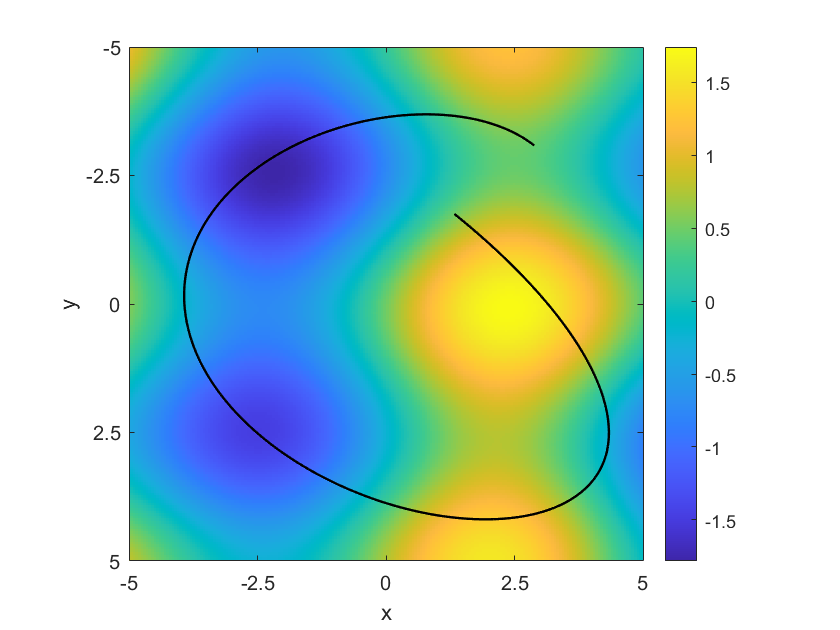
\includegraphics[width=0.5\textwidth]{../../Images/trajectoire.png}}
\caption{Trajectory of the system over the observation field}\label{fig:trajectoire}
\end{figure}

Four filters are evaluated over $N_{MC}=100$ Monte Carlo runs to solve the presented navigation problem:
\begin{itemize}
\item three PFs using a known but degraded observation function of the form:
\begin{equation}
H_\alpha(x)\triangleq(1+\varepsilon(x))\cdot H(x),\:\varepsilon(x)\sim\mathcal{N}(0,\alpha)
\end{equation}
with degradation levels $\alpha\in\{0,\:0.1,\:0.5\}$,
\item the RFF/RLS AKKF SLAM presented by algorithm \ref{alg:RFF/RLS AKKF SLAM}.
\end{itemize}

Each filter uses $1000$ particles. For the RKHS formulation, both kernels are chosen as Gaussian:
\begin{equation}
k(x,x')\triangleq\exp\left(-\frac{1}{2}\frac{||x-x'||_2^2}{1.5^2}\right)
\end{equation}
and the regularisation parameters are set to $\lambda_x=\lambda_z=0.1$. The RFF approximation is performed using $D=500$ features, with frequencies sampled from a Gaussian distribution $p(\omega)\sim\mathcal{N}(0,1.5)$. Finally, RLS is configured with a regularisation factor $\lambda_{RLS}=0.01$ and a forgetting factor $\beta=0.995$.

\subsection{SLAM Performance}

The root mean squared error (RMSE) of each filter at time step $k\in[\![1,N_{iter}]\!]$ is defined as:
\begin{equation}
\text{RMSE}_x(k)\triangleq\sqrt{\frac{\sum_{m=1}^{N_{MC}}||x_k-\hat{x}_{k,m}||_2^2}{N_{MC}}}\label{eq:RMSE_x}
\end{equation}
where $\hat{x}_{k,m}$ denotes the estimated state computed by the $m$-th Monte-Carlo run at time $k$. Figure \ref{fig:RMSE_x} gives the $\text{RMSE}_x$ curves of all four tested filters.

\begin{figure}[ht]
\centerline{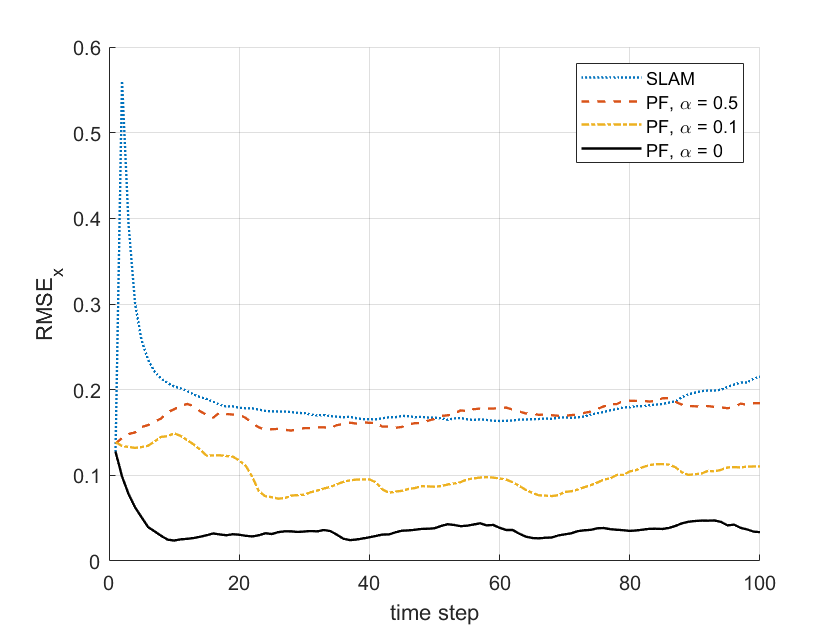
\includegraphics[width=0.5\textwidth]{../../Images/RMSE_x.png}}
\caption{$\text{RMSE}_x$ as a function of time for the studied filters}\label{fig:RMSE_x}
\end{figure}

Unsurprisingly, the $\text{RMSE}_x$ for the PFs decrease with $\alpha$, as the given observation function is increasingly precise. It must also be noted that with $\alpha=0.5$, the PF is only able to maintain the initial estimation error without being able to converge to lower errors as $\alpha=0.1$ and $\alpha=0$ do. On the other hand, while the state RMSE for RFF/RLS AKKF SLAM only reaches that of the most degraded PF, it is able to reduce its high early estimation error from $0.56$ at time step $k=5$ down to $0.19$ during the last $20$ iterations. This is due to the fact that algorithm \ref{alg:RFF/RLS AKKF SLAM} has to learn the observation model, while the other filters have direct access to an already known, albeit degraded, observation function $H_{\alpha}$. Table \ref{tab:RMSE_x ratio} computes the early stage maximum $\text{RMSE}_x$ to average final $\text{RMSE}_x$ for the four evaluated filters.

\begin{table}[ht]
\caption{Transient to asymptotic $\text{RMSE}_x$ comparison\\across the tested filters}\label{tab:RMSE_x ratio}
\centerline{\begin{tabular}{|c|c|c|c|c|}\hline
&SLAM&PF, $\alpha=0.5$&PF, $\alpha=0.1$&PF, $\alpha=0$\\\hline
Maximum $\text{RMSE}_x$&\multirow{2}{*}{$0.56$}&\multirow{2}{*}{$0.18$}&\multirow{2}{*}{$0.15$}&\multirow{2}{*}{$0.13$}\\
for $k\in[\![1,10]\!]$&&&&\\\hline
Mean $\text{RMSE}_x$&\multirow{2}{*}{$0.19$}&\multirow{2}{*}{$0.18$}&\multirow{2}{*}{$0.11$}&\multirow{2}{*}{$0.04$}\\
for $k\in[\![80,100]\!]$&&&&\\\hline
Early maximum/&\multirow{2}{*}{$2.88$}&\multirow{2}{*}{$0.96$}&\multirow{2}{*}{$1.38$}&\multirow{2}{*}{$3.15$}\\
late mean ratio&&&&\\\hline
\end{tabular}}
\end{table}

While the absolute $\text{RMSE}_x$ remains high for algorithm \ref{alg:RFF/RLS AKKF SLAM}, the transient to asymptotic ratio highlights a decrease of the estimation error for RFF/RLS AKKF SLAM similar to that of the PF with access to the perfect observation model. This suggests that the iterative learning of the observation model proposed by our method is able to reduce the long-term error, even when the early $\text{RMSE}_x$ is more pronounced.

Similarly to \eqref{eq:RMSE_x}, the reconstruction error of the observation function is evaluated through the spatial RMSE:
\begin{equation}
\text{RMSE}_z:x\in\mathbb{R}^2\mapsto\sqrt{\frac{\sum_{m=1}^{N_{MC}}||H(x)-\hat{H}_m(x)||_2^2}{N_{MC}}}
\end{equation}
where $\hat{H}_m$ denotes to the final estimation of the map by the $m$-th run of algorithm \ref{alg:RFF/RLS AKKF SLAM} as described by \eqref{eq:observation RFF}. Figure \ref{fig:carte_reconstruite} presents representative reconstruction of the observation function, while \ref{fig:RMSE_z} shows the spatial distribution of $\text{RMSE}_z$. Its average is $0.21$ over the $[-5,5]\times[-5,5]$ domain, reduced to $0.07$ along the true trajectory.

\begin{figure}[ht]
\centerline{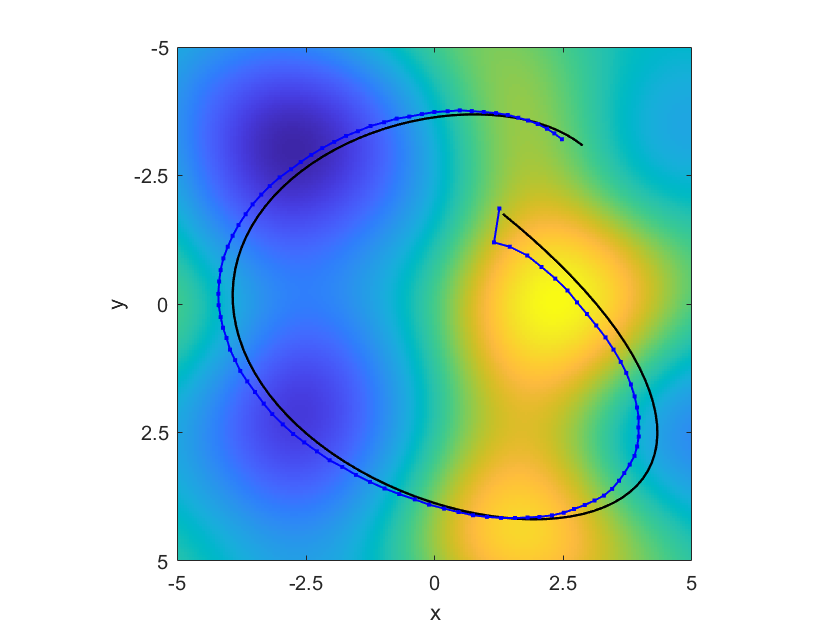
\includegraphics[width=0.5\textwidth]{../../Images/carte_reconstruite.png}}
\caption{An example of reconstructed observation function by algorithm \ref{alg:RFF/RLS AKKF SLAM} and its corresponding estimated trajectory in dotted blue}\label{fig:carte_reconstruite}
\end{figure}

\begin{figure}[ht]
\centerline{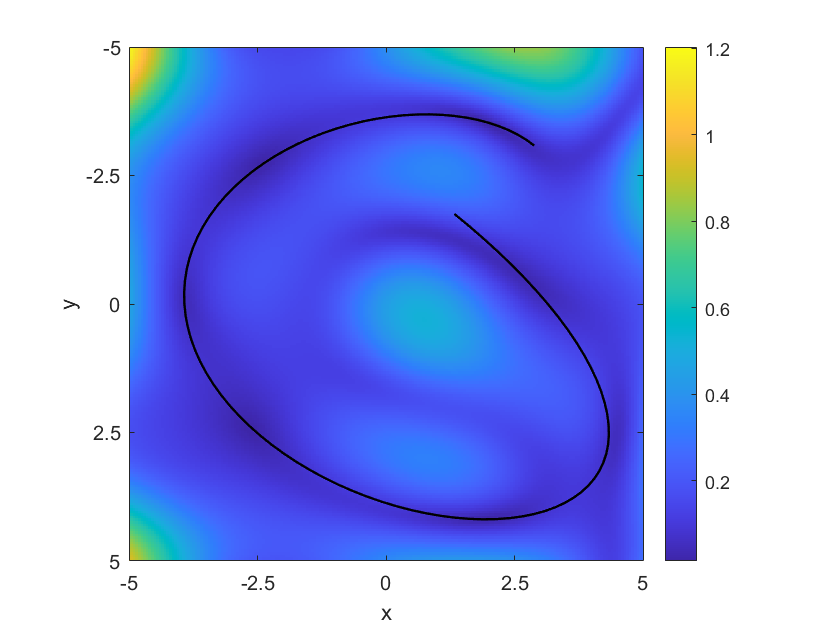
\includegraphics[width=0.5\textwidth]{../../Images/RMSE_z.png}}
\caption{Spatial distribution of the reconstruction error}\label{fig:RMSE_z}
\end{figure}

Four reconstruction error peaks can be observed in figure \ref{fig:RMSE_z}. Three of them are located on the exterior of the trajectory, and correspond to extrapolation errors that would likely be smaller if the state trajectory were to cover those regions. The fourth, comparatively smaller, peak is located near the inner portion of the trajectory, and should primarily be attributed to state estimation errors rather than intrinsic map regression errors. Since the RLS process depends explicitly on the estimated state $\hat{x}_k$, any localisation bias induces a spatial offset in the reconstructed observation field. Indeed, figure \ref{fig:carte_reconstruite} clearly shows a shifted reconstruction compared to figure \ref{fig:trajectoire} around the centre of the trajectory.

\section{Conclusion and Future Work}\label{sec:conclusion}

In this paper, we introduced a new simultaneous localisation and mapping (SLAM) framework that combines the Adaptive Kernel Kalman Filter (AKKF) with Random Fourier Features (RFF) and Recursive Least Squares (RLS) to jointly estimate the system state and learn the observation model in a fully recursive manner. By embedding both the state and observation spaces in Reproducing Kernel Hilbert Spaces (RKHS), the proposed approach extends the applicability of Kalman filtering to highly non-linear and non-injective systems, while enabling a recursive learning of the observation function.

Numerical results illustrate that, although the absence of a known observation function results in a larger initial estimation error, the proposed RFF/RLS AKKF SLAM progressively reduces both state and observation errors. The method achieves performance comparable to particle filtering approaches that assume partially known observation models. The spatial analysis of the reconstructed observation function further highlights the algorithm’s capability to accurately learn the underlying map along the explored trajectory.

Future work will focus on explicitly integrating state uncertainty into the map regression, investigating the joint estimation of observation parameters with the state, and validating the method on real-world applications.

\section*{Acknowledgement}

The authors would like to thank Dr. Athénaïs Gautier for her helpful discussions and clarifications.

\printbibliography

\end{document}
